\documentclass{ctexart}
\usepackage{graphicx}
\usepackage{caption}
\usepackage{float}
\usepackage{amsmath}
\usepackage{fancyhdr}
\usepackage{xunicode-addon}
\usepackage{booktabs}
\usepackage{listings}
\usepackage{hyperref}
\usepackage[a4paper,hmargin=1.25in,vmargin=1in]{geometry}
% !TeX program = xelatex
\lstdefinestyle{mystyle}{
  basicstyle=\ttfamily\footnotesize,
  breakatwhitespace=false,         
  breaklines=true,                 
  captionpos=b,                    
  keepspaces=true,                 
  numbers=left,                    
  numbersep=5pt,                  
  showspaces=false,                
  showstringspaces=false,
  showtabs=false,                  
  tabsize=2
}

\lstset{style=mystyle}

\title{\begin{figure}[H]
	\centering 
	\includegraphics[height=7cm,width=14cm]{E:/Pictures/中科大.jpg}
	\end{figure}\Huge\textbf{人工智能原理与技术}\\\huge{实验4}}
\date{}
\punctstyle{banjiao} 
\pagestyle{fancy}
	\fancyhead[C]{\LARGE\textbf{实验4}}
	\fancyhead[L]{}
	\fancyhead[R]{}
	\fancyfoot[C]{\thepage}
\begin{document}
	\maketitle
	\thispagestyle{empty}
	
	\[\makebox{\Large{姓名:\underline{\makebox[5cm]{高茂航}}}}\]
	
    \[\makebox{\Large{学号:\underline{\makebox[5cm]{PB22061161}}}}\]
	
	$$\makebox{\Large{日期:\underline{\makebox[5cm]{2024.7.6}}}}$$
	
	\clearpage

	\pagenumbering{arabic}

	\section{Torch配置}

	\begin{figure}[H]
		\centering 
		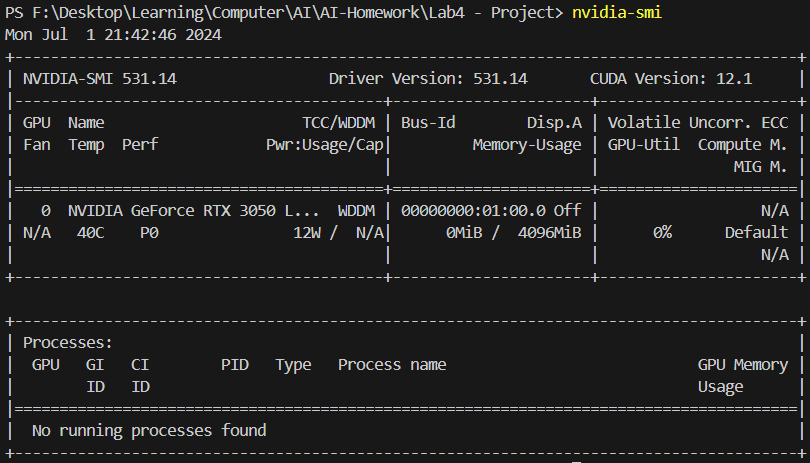
\includegraphics[height=5.5cm,width=10cm]{1.png}
		\end{figure}
		\begin{figure}[H]
			\centering 
			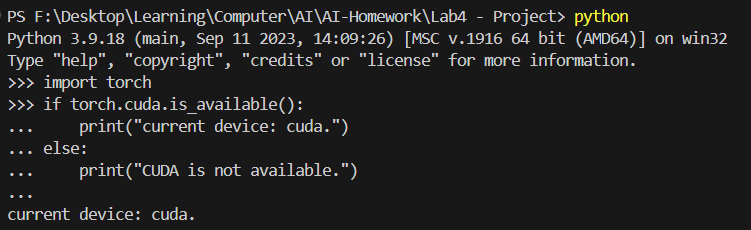
\includegraphics[height=3cm,width=10cm]{2.png}
			\end{figure}
	
	\section{实验原理}
\subsection{二元零和马尔可夫博弈}
一个涉及两个玩家在一系列状态中进行决策的过程,其中每个玩家的目标是最大化自己的累计奖励(或最小化对方的累计奖励),而这个过程的状态转移遵循马尔可夫性质。
在每个状态,玩家需要基于当前的信息选择最优策略,而这个选择会影响到游戏的下一个状态和玩家的即时奖励。由于是零和博弈,一个玩家的收益等于另一个玩家的损失,使得这种博弈具有高度的竞争性。
\subsection{Naive Self Play}
让AI与其自身的副本进行对战,通过这种方式根据自身经验不断学习适应并调整,以提高其性能。该方法较为简单直接,如果要避免不收敛等问题,需要采取更复杂的算法。
\subsection{Actor-Critic}

这种方法旨在通过同时学习一个策略(即Actor)和一个值函数(即Critic)来平衡探索和利用,从而提高学习效率和性能。
Actor根据当前策略选择动作,并执行该动作。Critic评估执行动作后的结果,即计算实际回报与预期回报之间的差异(TD误差)。
接着使用TD误差来更新Critic的值函数参数,使其预测更加准确。
最后根据Critic提供的反馈(TD误差),更新Actor的策略参数,以便在未来选择更好的动作。
\section{模型设计}
\begin{lstlisting}
	class Actor(nn.Module):
    def __init__(self, board_size: int, lr=1e-4):
        super().__init__()
        self.board_size = board_size
        # BEGIN YOUR CODE
        self.conv_blocks = nn.Sequential(
            nn.Conv2d(in_channels=1, out_channels=64, kernel_size=3, padding=1),
            nn.LeakyReLU(0.01),
            nn.Conv2d(in_channels=64, out_channels=128, kernel_size=3, padding=1),
            nn.LeakyReLU(0.01),
        )
        self.linear_blocks = nn.Sequential(
            nn.Linear(in_features=board_size ** 2 * 128, out_features=board_size ** 2),
            nn.LeakyReLU(0.01),
            nn.Dropout(0.5),
        )
        # END YOUR CODE

        # Define your optimizer here, which is responsible for calculating the gradients and performing optimizations.
        # The learning rate (lr) is another hyperparameter that needs to be determined in advance.
        self.optimizer = torch.optim.Adam(params=self.parameters(), lr=lr)

    def forward(self, x: np.ndarray):
        if len(x.shape) == 2:
            output = torch.tensor(x).to(device).to(torch.float32).unsqueeze(0).unsqueeze(0)
        else:
            output = torch.tensor(x).to(device).to(torch.float32)
		# BEGIN YOUR CODE
		# 将output中不合法的位置置为零
        x_flat = output.flatten(start_dim=2)
        mask = (x_flat == 0).float()
        
        output = self.conv_blocks(output)
        output = nn.Flatten()(output)
        output = self.linear_blocks(output)
        mask = mask.reshape(-1, self.board_size ** 2)
        output = output.reshape(-1, self.board_size ** 2)
        output = output * mask

		#以下几步解决output的归一化问题
        # 找出output中非零的位置
        non_zero_mask = output != 0
        # 把output中的零替换为一个很小的数
        output_adjusted = torch.where(non_zero_mask, output, torch.tensor(-1e10).to(output.device))
        # 对output_adjusted进行softmax操作
        softmax_output_adjusted = nn.functional.softmax(output_adjusted, dim=1)
        # 把softmax_output_adjusted中的非零位置的值替换回output中的值
        softmax_output_final  = torch.where(non_zero_mask, softmax_output_adjusted, output)
        output = softmax_output_final
        # END YOUR CODE

        return output


class Critic(nn.Module):
    def __init__(self, board_size: int, lr=1e-4):
        super().__init__()
        self.board_size = board_size
        # BEGIN YOUR CODE
        self.conv_layers = nn.Sequential(
            nn.Conv2d(in_channels=1, out_channels=64, kernel_size=3, stride=1, padding=1),
            nn.LeakyReLU(0.01),
            nn.Conv2d(in_channels=64, out_channels=128, kernel_size=3, stride=1, padding=1),
            nn.LeakyReLU(0.01),
            nn.Flatten(),
        )
        self.fc_layers = nn.Sequential(
            nn.Linear(in_features=board_size ** 2 * 128, out_features=board_size ** 2),
            nn.LeakyReLU(0.01),
            nn.Dropout(0.5),
        )
        # END YOUR CODE

        self.optimizer = torch.optim.Adam(params=self.parameters(), lr=lr)

    def forward(self, x: np.ndarray, action: np.ndarray):
        indices = torch.tensor([_position_to_index(self.board_size, x, y) for x, y in action]).to(device)
        if len(x.shape) == 2:
            output = torch.tensor(x).to(device).to(torch.float32).unsqueeze(0).unsqueeze(0)
        else:
            output = torch.tensor(x).to(device).to(torch.float32)

        # BEGIN YOUR CODE
        output = self.conv_layers(output)
        q_values = self.fc_layers(output)
        q_values = q_values.view(-1, self.board_size ** 2)
        output = q_values.gather(1, indices.unsqueeze(1)).squeeze(1)

        # END YOUR CODE

        return output
	\end{lstlisting}

		一开始采用如下结构,结果最后output全为0,胜率为0.53,原因可能是:
		
		(1)如果网络参数权重初始化过小,经过ReLU激活函数后,所有负值都会被置为0;
	
		(2)学习率设置不合理,可能导致网络权重在训练初期就更新到了一个不合理的范围,从而导致输出全为0;
	
		(3)在深层网络中,梯度可能会随着传播逐渐减小,最终导致梯度消失。
		
		将nn.ReLU()改为nn.LeakyReLU(0.01)并加上nn.Dropout(0.5)后output就正常了,
	上述问题可能主要是由第一个原因造成的。
	\begin{lstlisting}
		self.conv_layers = nn.Sequential(
			nn.Conv2d(in_channels=1, out_channels=64, kernel_size=3, stride=1, padding=1),
			nn.ReLU(),
			nn.Conv2d(in_channels=64, out_channels=128, kernel_size=3, stride=1, padding=1),
			nn.ReLU(),
			nn.Flatten(),
		)
		self.fc_layers = nn.Sequential(
			nn.Linear(in_features=board_size ** 2 * 128, out_features=board_size ** 2),
			nn.ReLU(),
		)
		\end{lstlisting}
	\section{constrained policy的解决思路}
具体过程在上一部分的forward部分代码中体现,主要是将非法位置置为0和归一化两部分。
前者一开始碰到的问题是理解错代码,以为每次都要加载一个棋盘,而不是处理x,导致报错;
后者的问题在于,假如对整个张量运用softmax函数,会导致非法位置归一化后不为0,而若只对合法位置归一化就很麻烦,
后来查了资料得知可以把非法位置的值替换为一个很小的负数,然后再对整体进行softmax操作,这样操作后非法位置还是0。
	\section{optimize函数中2个bug的的解决方案}
	在actor\_loss.backward()和critic\_loss.backward()后面分别加上
	self.actor.optimizer.step()和self.critic.optimizer.step(),
	因为这两对操作分别完成了actor和critic网络的梯度计算和参数更新,
	确保了每次迭代中,模型的参数都能根据损失函数的反向传播结果进行有效更新。

	\section{其他bug及解决方案}
	\begin{figure}[H]
		\centering 
		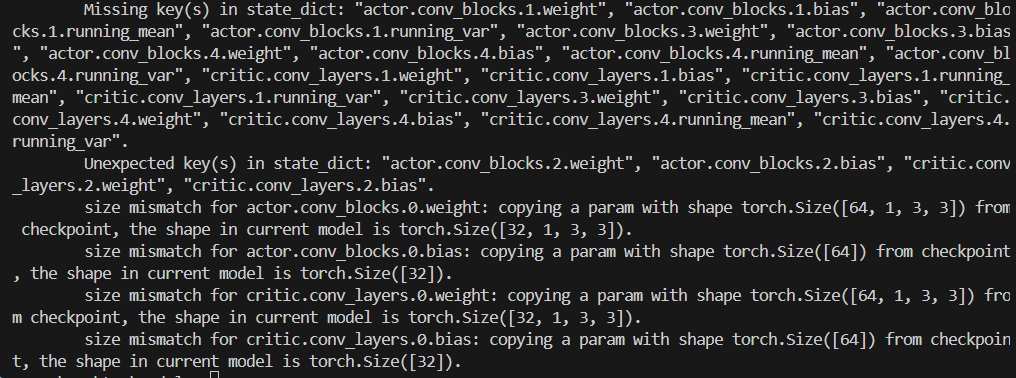
\includegraphics[height=4cm,width=10cm]{3.png}
		\end{figure}
		这个bug出现在opponent\_loader.py中加载的模型结构不对时,
		由于当时在evaluator.py中把random\_response设为True,以为这样就不用管opponent\_loader.py了,结果就发生了报错。

		此外,在训练过程时偶尔会因为内存溢出而导致训练终止,一般要通过中止进程或重启来解决。
	\section{难以理解的点及解释}
	不太清楚的是保存到model.pth文件的模型是什么形式的,后来阅读代码和查阅资料后了解到训练并保存的模型是一个PyTorch模型的状态字典(state dictionary)。
	状态字典包含了模型中所有可训练参数(如权重和偏置)的映射。当使用torch.save(model.state\_dict(), f"checkpoints/model\_\{\_\}.pth")保存模型时,
	它不会保存模型的结构,只保存参数。这意味着在加载模型时,需要先定义模型的结构,然后才能加载这些参数。
	.pth格式的文件是PyTorch的一种常用文件格式,一般用于存储模型参数。
	\section{loss 和 entropy 曲线分析}
	Actor的Loss含义: Actor的任务是根据当前状态选择动作,其目标是最大化期望奖励。Actor的loss通常是基于策略梯度的,意在评估所选动作与最优动作之间的差距。这个loss的计算通常涉及到所选择动作的概率和这个动作带来的预期回报(或优势)。我们希望最大化这个预期回报,但在优化过程中,我们实际上是最小化一个负的期望回报(即最大化期望回报的负数形式),这样做是为了符合常规优化问题的形式,即最小化loss。

Critic的Loss含义: Critic的任务是评估当前状态或动作的价值,
即预测从当前状态开始,采取特定动作能获得的期望回报。Critic的loss是基于值函数的预测误差,通常是时间差分(TD)误差或均方误差。这个误差衡量了Critic的预测值与实际获得的回报之间的差异。我们希望这个误差尽可能小,这意味着Critic的预测越准确越好。

	在Actor-Critic架构中,policy对应的熵是一个衡量policy随机性的指标。
	熵越高,表明policy的行为选择越随机;熵越低,表明policy的行为选择越确定性。
	在强化学习中,较高的熵有助于探索,可以防止算法过早地收敛到局部最优解,
	而较低的熵有助于算法在找到好的策略后稳定执行。因此,在训练初期,我们可能希望保持较高的熵以鼓励探索;在训练后期,当我们希望算法开始利用已学习的策略时,可能会逐渐降低熵的值。
	
	

		
	\section{对网络参数和结构的一些尝试}
	上述模型的相关图像如下:
	\begin{figure}[H]
		\centering 
		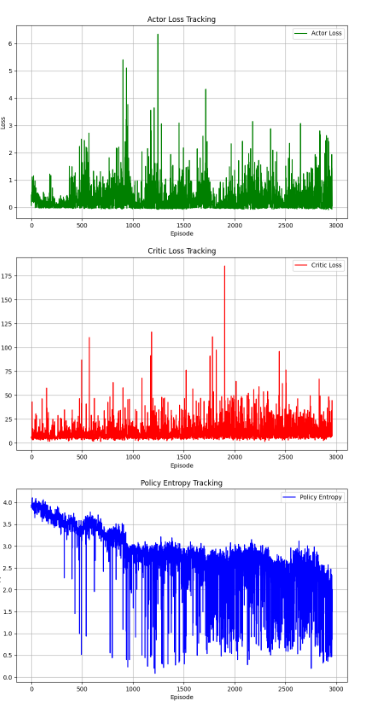
\includegraphics[height=10cm,width=6cm]{5.png}
		\end{figure}
		为了叙述方便,以下将该模型记为模型1,它和随机噪声对弈的胜率为1,和自己对弈的胜率约为0.5。
	
		试着把优化器换成随机梯度下降优化器(SGD),结果胜率明显下降,原因可能如下:
	Adam优化器结合了具有自适应学习率的特性,这使得它在很多情况下都能比较快速地收敛,并且对学习率的初始选择不是特别敏感。Adam优化器能够通过计算梯度的一阶矩估计和二阶矩估计来调整每个参数的学习率,使得它在训练初期和面对稀疏梯度时表现更好。
相比之下,SGD优化器通过对每个参数更新时使用固定的学习率来进行梯度下降。虽然SGD在很多简单问题上表现良好,但在处理复杂的非凸优化问题或是深度神经网络时,由于缺乏自适应学习率调整,可能需要更多的时间来调整学习率和其他超参数以达到良好的收敛效果。此外,SGD对于稀疏数据或是在训练初期可能不如Adam那样表现出色。

此外还试了RMSprop优化器,该优化器结合了梯度平方的指数衰减平均调整学习率,适合处理非平稳目标,但对于本实验的效果略差于Adam优化器。

尝试了将模型1的学习率改为1e-5(记为模型2),相关图像如下:
	\begin{figure}[H]
		\centering 
		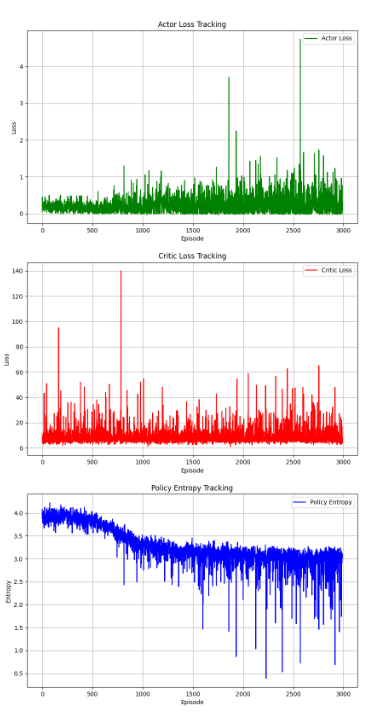
\includegraphics[height=10cm,width=6cm]{6.png}
		\end{figure}
	模型2和随机噪声对弈的胜率为0.991,和自己对弈的胜率为0.524,模型2(先手)和模型1对弈先手胜率为0.832,模型1(先手)和模型2对弈先手胜率为0.253,
	可见模型2由于模型1(故提交的也是模型2),运行player.py发现模型2是一直自顾自地连成一条直线而不去管对方,目前还不清楚这种策略是否有较好的泛化性能。

也尝试了把网络改为1,32,128的结构(记为模型3),相关图像如下:
	\begin{figure}[H]
		\centering 
		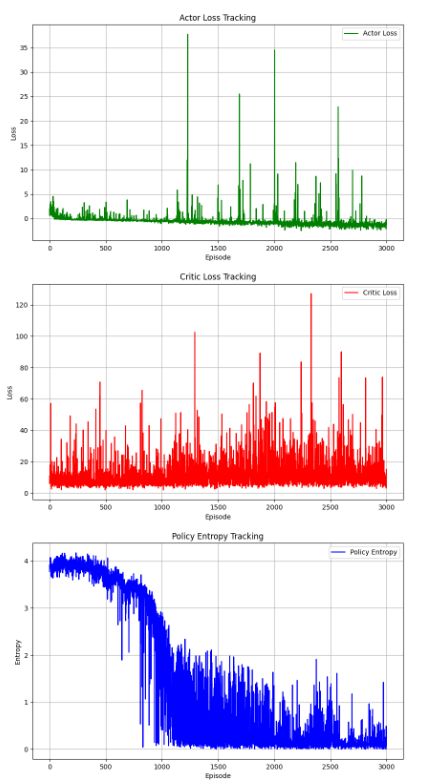
\includegraphics[height=10cm,width=6cm]{8.png}
		\end{figure}
模型3和随机噪声对弈的胜率为0.936,和自己对弈的胜率为0.789。
	
还尝试把模型4的学习率改为1e-5,相关图像如下:
	\begin{figure}[H]
		\centering 
		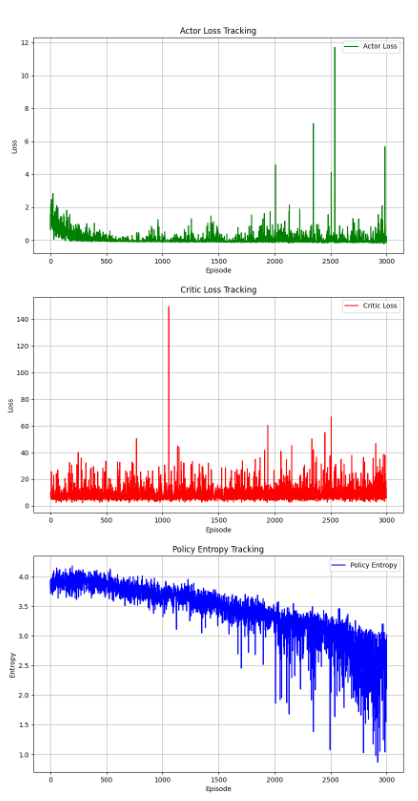
\includegraphics[height=10cm,width=6cm]{9.png}
		\end{figure}
		模型4和随机噪声对弈的胜率为0.822,和自己对弈的胜率为0.525。总的来说模型3,4不如模型1,2的效果好。

后来试着写了前馈神经网络(FNN)和循环神经网络(RNN)等,均由于对相关内容还不够熟悉,没能调试成功,最后尝试了transformer,效果稍好于前述的CNN的模型,但训练的时间更长,相关图像如下:
	\begin{figure}[H]
		\centering 
		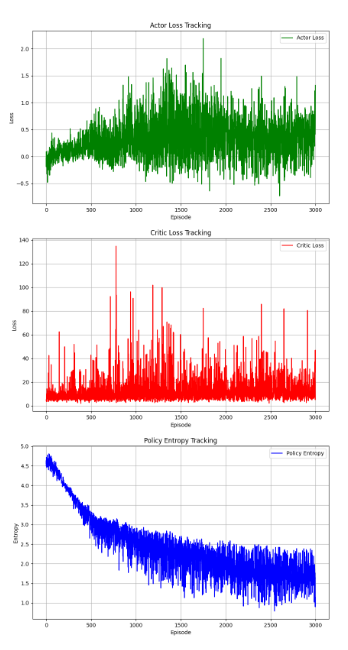
\includegraphics[height=10cm,width=6cm]{4.png}
		\end{figure}
可见熵的曲线下降较快,而与上述其他图像差异最大的地方是actor loss在训练中后期较为均匀,且出现了负值。

	此外本来还想增加迭代次数,但由于时间关系没能实现。一开始还碰到的一个问题是发现不同网络训练出来的模型不能直接对弈,后来发现是因为模型的参数不同,需要在opponent\_loader.py里载入正确的模型结构。
	\section{思考题}
	在最理想的情况下,即使模型的权重收敛到使得actor loss和critic loss最优的点,黑棋和白棋双方的策略也不一定达成纳什均衡,原因如下:

(1)纳什均衡指的是在一个非合作博弈中,每个参与者选择的策略使得在其他参与者的策略给定的情况下,自己的策略最优,这意味着在纳什均衡点,没有任何一个参与者可以通过单方面改变自己的策略来获得更好的结果。
而actor loss和critic loss的最优化目标是最小化预测误差和提高决策的准确性,这与博弈论中的策略最优化不完全相同;

(2)模型权重的收敛到最优点意味着在给定的训练数据和模型结构下,模型找到了一组参数,这组参数能够最小化loss函数。然而,这并不保证模型找到的是全局最优解,也不保证这个最优点就对应着纳什均衡。特别是在复杂的环境和策略空间中,存在多个局部最优解,而这些局部最优解可能并不对应于纳什均衡;

(3)在实际的博弈中,环境可能是动态变化的,参与者的策略也可能随时间变化。即使模型在某一时刻达到了loss的最优,也不能保证这个状态在环境变化后仍然是最优的,此外,实际环境中的不确定性和信息的不完全性也可能阻碍达成纳什均衡;

(4)纳什均衡的达成依赖于所有参与者策略的相互适应。即使一个参与者找到了自己的最优策略,如果其他参与者的策略改变,那么原来的最优策略可能不再是最优的。因此,即使模型找到了最优的loss点,也需要所有参与者的策略共同适应才能达到纳什均衡。
	\section{课程反馈}

本课程较好地锻炼了代码能力,加深了对人工智能常见算法的理解。虽然每次实验都感觉比较难,每次至少要花费整整几天的时间,
但做下来还是很有收获,也提高了debug和独立思考的能力,感到特别困难的部分还是集中在数学推导方面。

	

\end{document}